\documentclass[11pt, a4paper]{report}

\usepackage[utf8]{inputenc}
\usepackage[german, english]{babel} 
\usepackage{amsmath}
\usepackage{amsfonts}
\usepackage{amssymb}
\usepackage{epigraph}

\usepackage{setspace} %linespacing
\onehalfspacing

\usepackage[top=1in, bottom=1in, left=1.25in, right=1in]{geometry} %setting merges

\usepackage[T1]{fontenc}
\usepackage{graphicx}
\usepackage{lmodern}
\usepackage{caption}
\usepackage{siunitx}
\usepackage{tabularx}
\usepackage{listings}
\usepackage{hyphenat}
\usepackage{pdfpages} %including pdfs
\usepackage{chemfig} % drawing chemical figures
\usepackage{gensymb} % \degree symbol
\usepackage{float} %placing floats(H)

\graphicspath{{/home/thiele/Documents/Physik/HiWi/WW/Plots/}}


\begin{document}
\section*{MD simulation of the WW-loop}
This paper summarizes some results of the investigation of energy flow in
the WW-loop using MD simulations.  The target system is the modified WW loop with
34 residues, where residuum 19 was substituted with azulenylalanine (AZU) and
residue 8 was substitued with azidohomoalanine (AHA). AZU
can in experiment be excited at a typical wavelength of 600\,nm and decays on
the sub-picosecond timescale due to internal conversion. Because of this it is well
suited to pump energy into the system. AHA has a typical vibrational band at
2100\,cm$^{-1}$ which is separable in the IR spectrum. The AHA-AZU pair is thus
well suited for pump-probe-spectroscopy of vibrational energy transport in the
WW-loop \cite{C3CP54760D}.\\


The goal of the herein evaluated simulations was to model the heating of AHA and
observe the vibrational energy transport through the protein. The simulation
flow is the following: 
All simulations are performed with the GROMACS program suite \cite{GROMACS13}.
and the AMBER99sb*-ildn force field is used to model the WW-loop and the TIP3P water.\\
To couple the system to
the heat bath, we use the velocity-rescale algorithm \cite{Bussi07}, and for
pressure
coupling the Berendsen algorithm\cite{Berendsen84}. In the beginning the protein was inserted in a dodecahedron box. For the
simulation in solvent we add about 1600 water molecules. For the hydrated
system we use the Particle-Mesh Ewald method\cite{Darden93} for the
electrostatic
interactions beyond a miniamal cut-off of 1.4 nm and for the van der Waals
interaction a plain cut off at 1.4 nm. 
After energy minimization, the system is equilibrated for 100 ns at a pressure
of 1 atm and a temperature of 100
K. From the second half of this simulation we
obtained the average box size for the followed NVT simulation. \\
We then take 200 statistically
independent conformations from a 100 ns 100 K NVT simulation as starting
structures for the non-equilibrium simulations.
All the starting structures were cooled down to 10 K using a NPT ensemble to
improve
the signal to noise ratio of the following nonequilibrium simulation. \\

For the excitation with T-jump method we first freeze out all degrees
of freedom of the system except for the chromophore of residue AZU 19.
The chromophore is then coupled to a 910\,K bath and heated for 1\,ps.
Following the heating step the velocities of
the frozen atoms are set back to the velocities of the corresponding
equilibrium step.\\ 

Finally the non-equilibrium simulations of all 200 structures were run in a NVE ensemble for 100\,ps
each, using a timestep of 0.2\,fs. The time evolution of the kinetic energy of
all residues was averaged over all 200 trajectories and is shown in the plots
below.  

\section{Results in total kinetic energiy}
\begin{figure}[h]
  \centering
  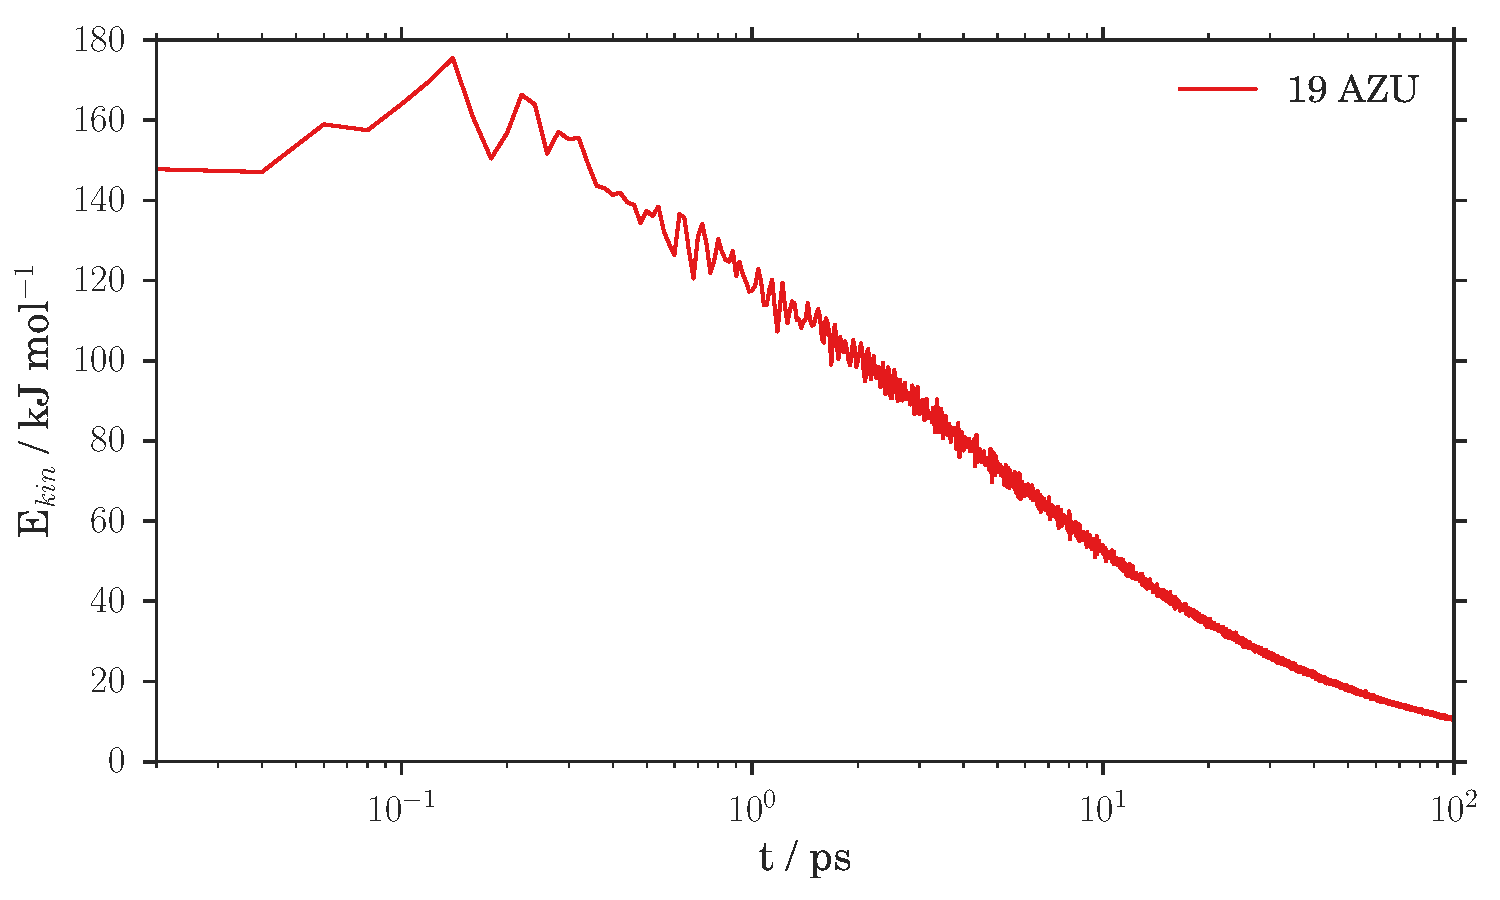
\includegraphics[width=0.8\linewidth]{E_kin_MD_19AZU.pdf}
  \caption{Kinetic energy of the heated residuum AZU 19. The characteristic time
    of decay between 0.2\,ps and 40\,ps obtained from fitting is $\tau_{AZU}
  \approx$ 10\,ps.}
  \label{fig:E_kin_MD_19}
\end{figure}

\begin{figure}[h]
  \centering
  \includegraphics[width=0.8\linewidth]{E_kin_MD_7GLU_8AHA_9ARG.pdf}
  \caption{Kinetic energy of residues 7 GLU, 9 ARG and the possible thermometer
  8 AHA. The maximum rise in the kinetic energy of 8 AHA is around three times smaller
than that of the direct neighbour of AZU 18 TYR. The energies are normalized to the value at $t=0$. }
  \label{fig:E_kin_MEQ_9ARG_10MET_11SER_12ARG}
\end{figure}

\begin{figure}[h]
  \centering
  \includegraphics[width=0.8\linewidth]{E_kin_MD_14SER_15GLY_16ARG_17VAL_18TYR.pdf}
  \caption{Kinetic energy of downstream residues 14 to 18. The energies are
  normalized to the value at $t=0$.}
  \label{fig:E_kin_MD_15_16_17_18}
\end{figure}

\begin{figure}[h]
  \centering
  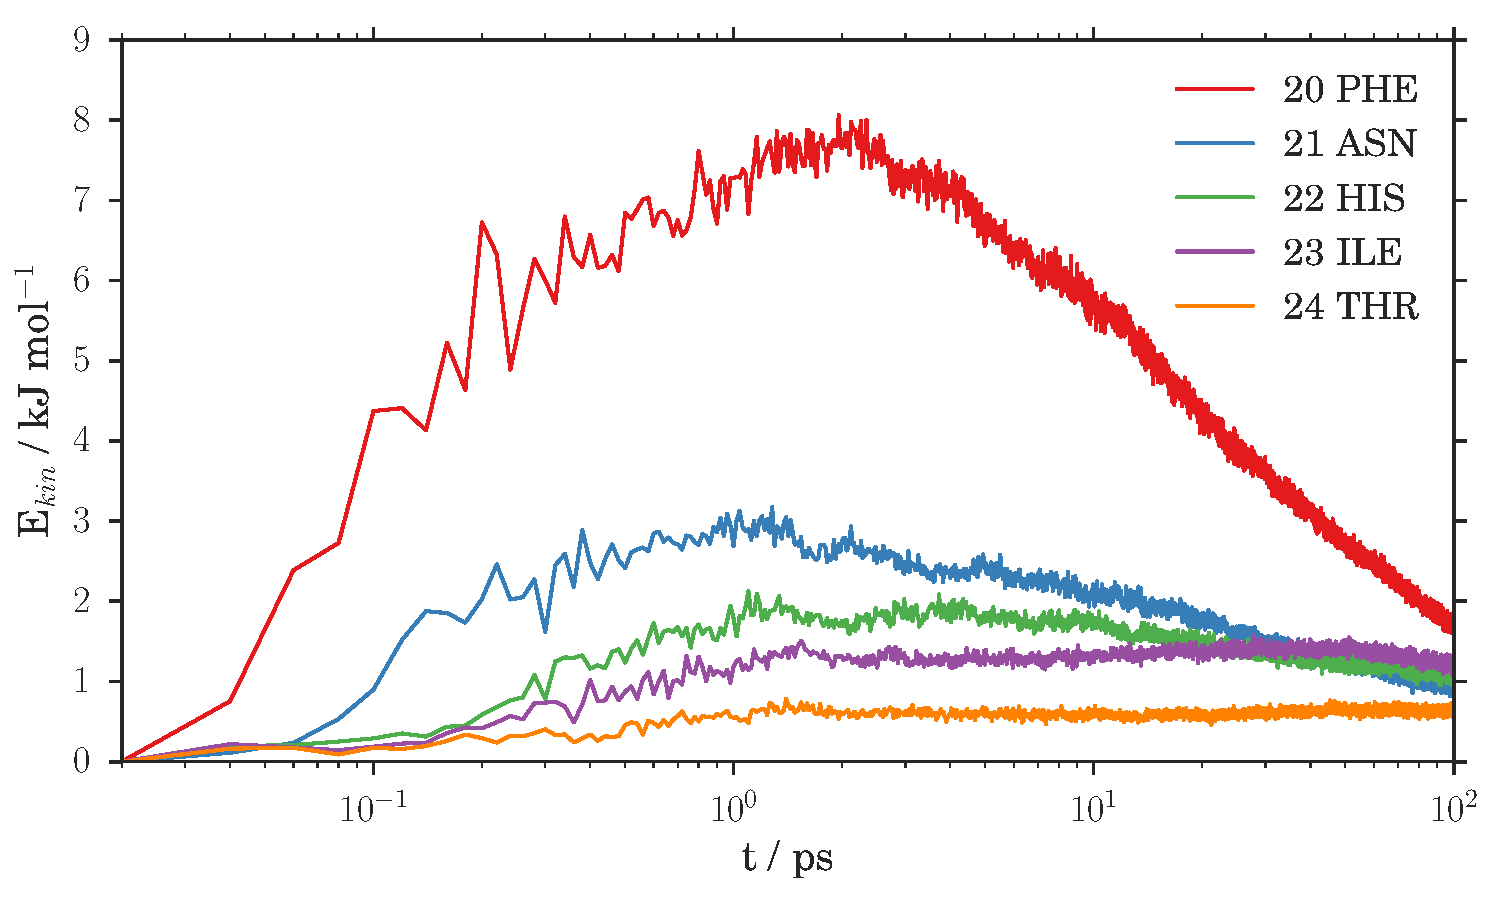
\includegraphics[width=0.8\linewidth]{E_kin_MD_20PHE_21ASN_22HIS_23ILE_24THR.pdf}
  \caption{Kinetic energy of upstream residues 20 to 24.The energies are normalized to the value at $t=0$.}
  \label{fig:E_kin_MD_20_21_22_23}
\end{figure}

\begin{figure}[h]
  \centering
  \includegraphics[width=0.8\linewidth]{E_kin_MD_25ASN_26ALA_27SER.pdf}
  \caption{Kinetic energy of residues 25 ASN, 26 ALA and 27 SER. The energy
  dose for 26 ALA, which is a possible thermometer position, is one order of
magnitude smaller than the energy rise of 8 AHA. The energies are normalized to
the value at $t=0$.}
  \label{fig:name}
\end{figure}

\begin{figure}[h]
  \centering
  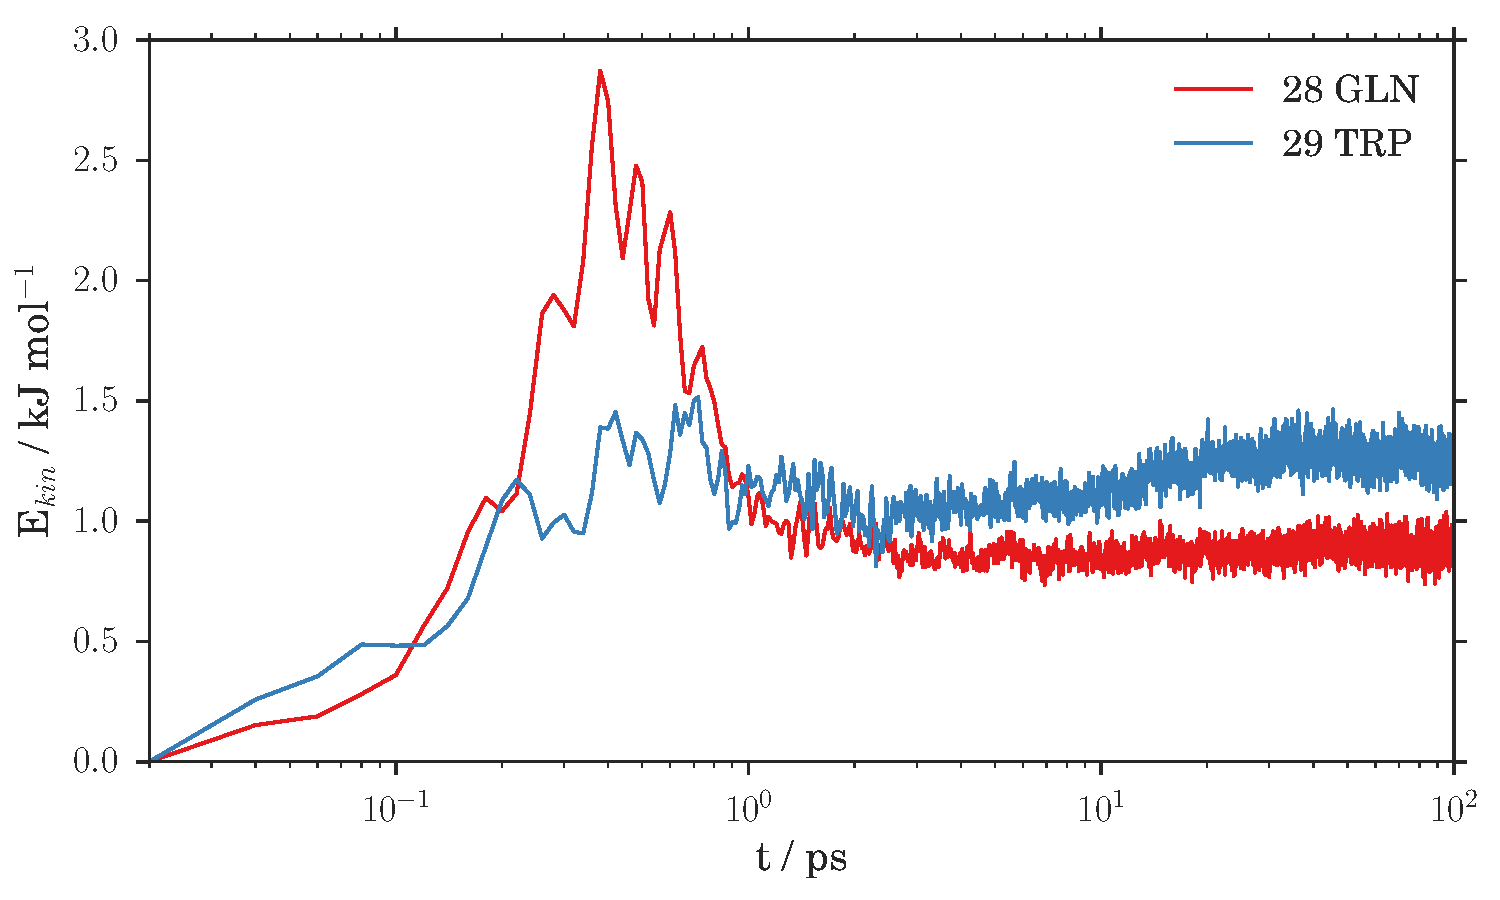
\includegraphics[width=0.8\linewidth]{E_kin_MD_28GLN_29TRP_30GLU_31ARG_32PRO_33SER_34GLY.pdf}
  \caption{Kinetic energy of residues 28 till end, of which 28 is in polar contact
  with 19 AZU. The energies are normalized to the value at $t=0$.}
  \label{fig:E_kin_MD_28GLN_29TRP_30GLU_31ARG_32PRO_33SER_34GLY}
\end{figure}

\section{Results in kinetic energy per dof}

\begin{figure}[h]
  \centering
  \includegraphics[width=0.8\linewidth]{E_kin_MD_dof_19AZU.pdf}
  \caption{Kinetic energy per dof of the heated residuum AZU 19. The characteristic time
    of decay between 0.2\,ps and 40\,ps obtained from fitting is $\tau_{AZU}
  \approx$ 10\,ps.}
  \label{fig:E_kin_MD_dof_19}
\end{figure}

\begin{figure}[h]
  \centering
  \includegraphics[width=0.8\linewidth]{E_kin_MD_dof_7GLU_8AHA_9ARG.pdf}
  \caption{Kinetic energy per dof of residues 7 GLU, 9 ARG and the possible thermometer
  8 AHA. The maximum rise in the kinetic energy of 8 AHA is around three times smaller
than that of the direct neighbour of AZU 18 TYR. The energies are normalized to the value at $t=0$. }
  \label{fig:E_kin_MEQ_9ARG_10MET_11SER_12ARG}
\end{figure}

\begin{figure}[h]
  \centering
  \includegraphics[width=0.8\linewidth]{E_kin_MD_dof_14SER_15GLY_16ARG_17VAL_18TYR.pdf}
  \caption{Kinetic energy per dof of downstream residues 14 to 18. The energies are
  normalized to the value at $t=0$.}
  \label{fig:E_kin_MD_dof_15_16_17_18}
\end{figure}

\begin{figure}[h]
  \centering
  \includegraphics[width=0.8\linewidth]{E_kin_MD_dof_20PHE_21ASN_22HIS_23ILE_24THR.pdf}
  \caption{Kinetic energy per dof of upstream residues 20 to 24.The energies are normalized to the value at $t=0$.}
  \label{fig:E_kin_MD_dof_20_21_22_23}
\end{figure}

\begin{figure}[h]
  \centering
  \includegraphics[width=0.8\linewidth]{E_kin_MD_dof_25ASN_26ALA_27SER.pdf}
  \caption{Kinetic energy per dof of residues 25 ASN, 26 ALA and 27 SER. The energy
  dose for 26 ALA, which is a possible thermometer position, is one order of
magnitude smaller than the energy rise of 8 AHA. The energies are normalized to
the value at $t=0$.}
  \label{fig:name}
\end{figure}

\begin{figure}[h]
  \centering
  \includegraphics[width=0.8\linewidth]{E_kin_MD_dof_28GLN_29TRP_30GLU_31ARG_32PRO_33SER.pdf}
  \caption{Kinetic energy per dof of residues 28 till end, of which 28 is in polar contact
  with 19 AZU. The energies are normalized to the value at $t=0$.}
  \label{fig:E_kin_MD_dof_28GLN_29TRP_30GLU_31ARG_32PRO_33SER_34GLY}
\end{figure}
\clearpage

\bibliography{md,stock,own}{}
\bibliographystyle{aip+title}

\end{document}
